\documentclass[12pt,letterpaper]{book}

\usepackage[utf8]{inputenc}
\usepackage[T1]{fontenc}
\usepackage{lmodern}
\usepackage[margin=1.25in,headheight=15pt]{geometry}
\usepackage{amsmath,amsthm,amssymb}
\usepackage{enumitem}
\usepackage{hyperref}
\usepackage{fancyhdr}
\usepackage{csquotes}
\usepackage{titlesec}
\usepackage{setspace}
\usepackage{listings}
\usepackage{xcolor}
\usepackage{graphicx}

% Spacing
\onehalfspacing

% Code listing style
\definecolor{codegreen}{rgb}{0,0.6,0}
\definecolor{codegray}{rgb}{0.5,0.5,0.5}
\definecolor{codepurple}{rgb}{0.58,0,0.82}
\definecolor{backcolour}{rgb}{0.95,0.95,0.92}

\lstdefinestyle{mystyle}{
    backgroundcolor=\color{backcolour},
    commentstyle=\color{codegreen},
    keywordstyle=\color{magenta},
    numberstyle=\tiny\color{codegray},
    stringstyle=\color{codepurple},
    basicstyle=\ttfamily\footnotesize,
    breakatwhitespace=false,
    breaklines=true,
    captionpos=b,
    keepspaces=true,
    numbers=left,
    numbersep=5pt,
    showspaces=false,
    showstringspaces=false,
    showtabs=false,
    tabsize=2
}

\lstset{style=mystyle}

% Chapter and section formatting
\titleformat{\chapter}[display]
  {\normalfont\huge\bfseries\centering}
  {\chaptertitlename\ \thechapter}{20pt}{\Huge}
\titleformat{\section}
  {\normalfont\Large\bfseries\centering}
  {\thesection}{1em}{}
\titleformat{\subsection}
  {\normalfont\large\bfseries}
  {\thesubsection}{1em}{}

% Spacing around titles
\titlespacing*{\chapter}{0pt}{50pt}{40pt}
\titlespacing*{\section}{0pt}{30pt}{20pt}
\titlespacing*{\subsection}{0pt}{20pt}{10pt}

% Header and footer setup
\pagestyle{fancy}
\fancyhf{}
\fancyhead[LE,RO]{\thepage}
\fancyhead[RE]{\textit{NeetCode 150}}
\fancyhead[LO]{\textit{Andre Ruiz Loera}}
\renewcommand{\headrulewidth}{0.4pt}

% Theorem environments
\newtheorem{theorem}{Theorem}
\newtheorem{proposition}{Proposition}
\theoremstyle{definition}
\newtheorem{definition}{Definition}
\theoremstyle{remark}
\newtheorem{remark}{Remark}
\newtheorem{note}{Note}

\hypersetup{
    colorlinks=true,
    linkcolor=blue,
    filecolor=magenta,
    urlcolor=cyan,
    pdftitle={NeetCode 150 - Commentary},
    pdfauthor={Andre Ruiz Loera},
}

\begin{document}

% Title page
\begin{titlepage}
\begin{center}

\vspace*{4cm}

{\Huge\bfseries NeetCode 150}\\[1cm]

{\Large\bfseries Solutions \& Commentary}

\vfill

{\LARGE Andre Ruiz Loera}

\vspace{3cm}

\end{center}
\end{titlepage}

% Preface (before TOC)
\chapter*{Preface}
\addcontentsline{toc}{chapter}{Preface}

I am a Mathematics major at the University of Illinois Urbana-Champaign and I have always enjoyed solving puzzles. Math gives you the peaceful kind of puzzle where you sit with an idea long enough and eventually something clicks. It is slow and thoughtful and satisfying when the pieces finally fall into place.

Coding feels different. It is still a puzzle but it is a louder one. And writing code in C++ feels like trying to solve a puzzle while you are on fire. It can be chaotic and confusing and still incredibly rewarding when it works. For a long time I actually became pretty good at the classic LeetCode style of problems. I had a sense for patterns and techniques and I could look at a question and feel the solution forming before I even finished the prompt.

Then I stopped for a while.

Life shifted toward other things and I did not work on these kinds of problems for months. When I returned I realized that my old LeetCode instincts had mostly evaporated. The skills were not gone forever but they were definitely sleeping. I felt like I had to start fresh again.

This book is my return to that world. It is my way of rebuilding my problem solving instincts one step at a time. The NeetCode 150 list is one of the clearest and most thoughtful collections of interview problems I know. Every problem teaches something specific and every solution strengthens a part of your thinking.

My goal in writing this is simple. I want to explain how I approach each problem. I want to write out the thought process the honest confusion the small breakthroughs and the cleanest version of a C++ solution that I can manage. I want this book to feel like you are sitting next to someone who is also working through these problems and talking through each idea as it forms.

If you are reading this I hope you find something helpful. Maybe a new way to look at a problem or the reassurance that you are not the only one who gets stuck sometimes. This is my journey back to algorithmic thinking and I am treating every problem as a chance to get sharper again.

Welcome to the process. And good luck. May your solutions arrive faster than they did for me when I first picked this back up.

\section*{What is NeetCode 150 and Why Use It}

The NeetCode 150 list is a curated set of one hundred and fifty coding interview problems gathered from the most common patterns that appear in technical interviews. It was created by NeetCode, a well-respected educator whose videos and write-ups focus on building real understanding rather than just memorizing tricks.

The list is organized by topic and by problem pattern. Each problem represents a skill that shows up repeatedly in interviews. For example sliding window, binary search, graph traversal, dynamic programming and many others. Because the list is structured and selective it gives you a very efficient way to study. You spend time on the problems that matter the most instead of trying to solve thousands of random questions with unclear purpose.

People use the NeetCode 150 to prepare for coding interviews at all levels. It covers the core ideas that interviewers expect candidates to know. It builds intuition about data structures and algorithms and it makes you better at recognizing patterns and adapting them to new problems.

I am using it because it is one of the most focused and effective paths back into algorithmic problem solving. It gives me a defined starting point and a clear progression. Working through the list forces me to practice thinking clearly under constraints and it gives me a chance to rebuild confidence and speed in a structured way.

In short the NeetCode 150 is a well-designed roadmap. It teaches the fundamentals that matter and prepares you for the type of reasoning that technical interviews and real-world problem solving require.

\clearpage

\section*{The Learning Roadmap}

The NeetCode 150 follows a structured progression that builds fundamental skills before advancing to more complex patterns. The roadmap below illustrates how topics connect and build upon each other:

\begin{figure}[h]
\centering
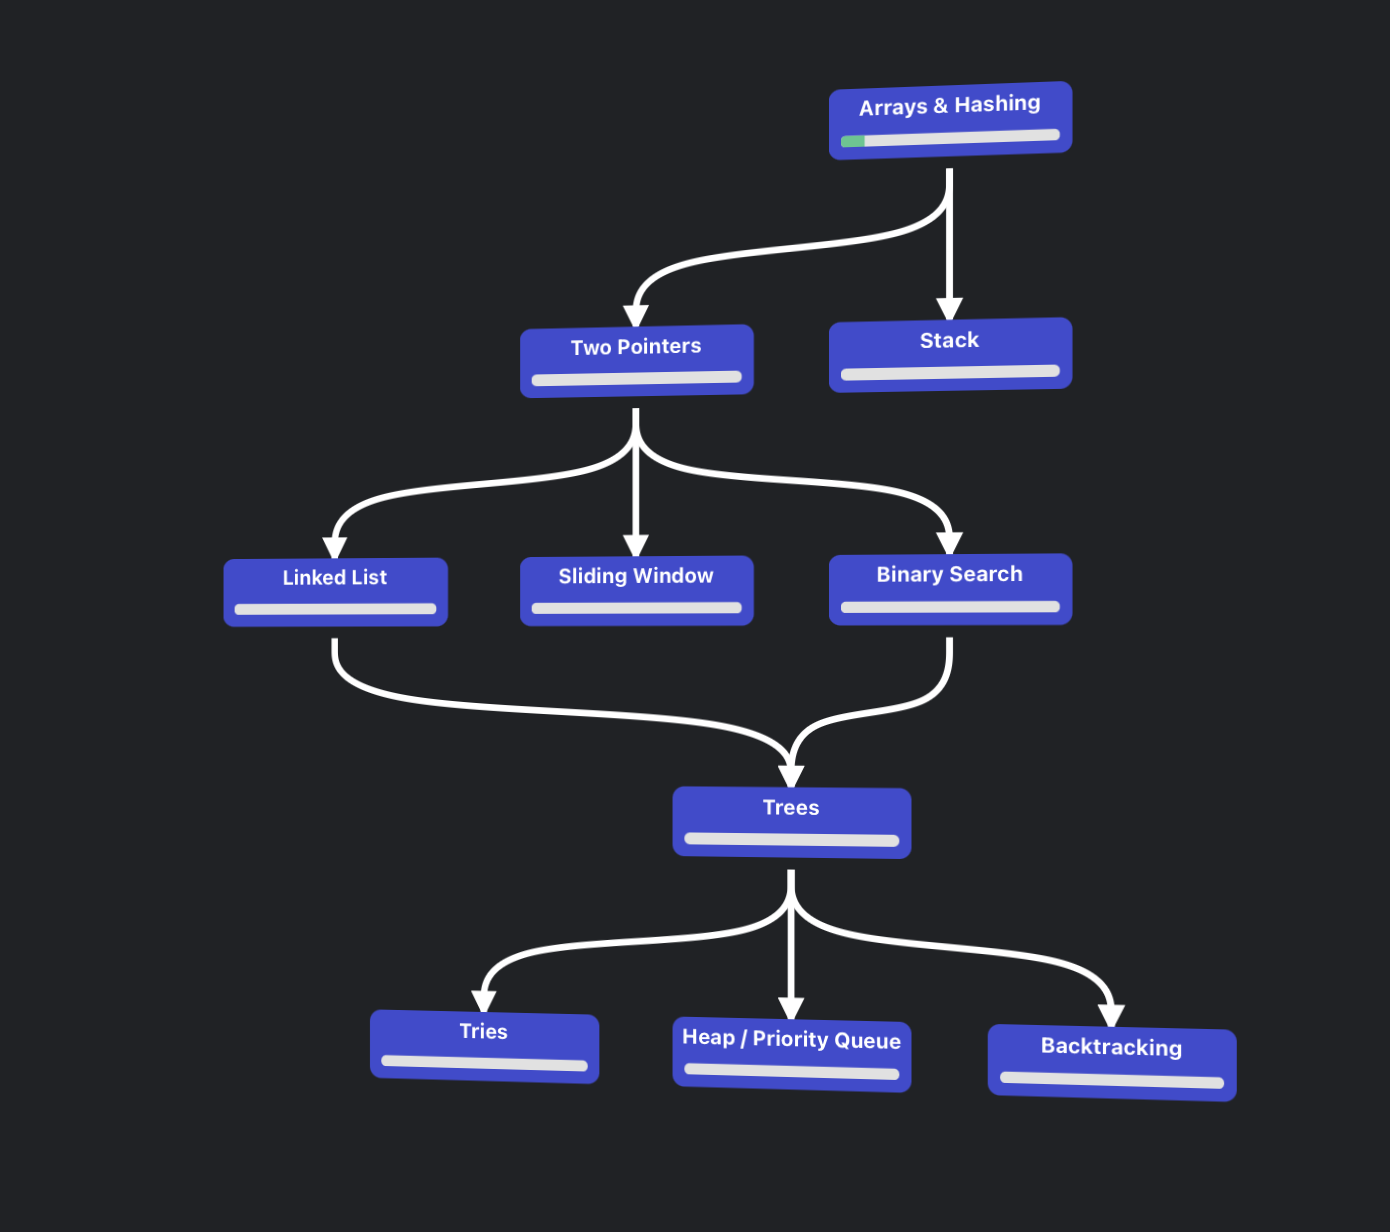
\includegraphics[width=0.9\textwidth]{neetcode-roadmap.png}
\caption{NeetCode 150 Learning Roadmap - Topic Progression}
\label{fig:roadmap}
\end{figure}

This visual guide shows the recommended path through the problems. Starting with Arrays \& Hashing establishes the foundation, then branching into Two Pointers and Stack techniques. From there, the path expands to cover Linked Lists, Sliding Window, and Binary Search. These foundational topics converge into Trees, which then branches into more specialized areas like Tries, Heaps, and Backtracking.

\clearpage

% Table of Contents
\tableofcontents
\clearpage

\chapter{Arrays \& Hashing}

\section{Contains Duplicate}

\begin{figure}[h]
\centering
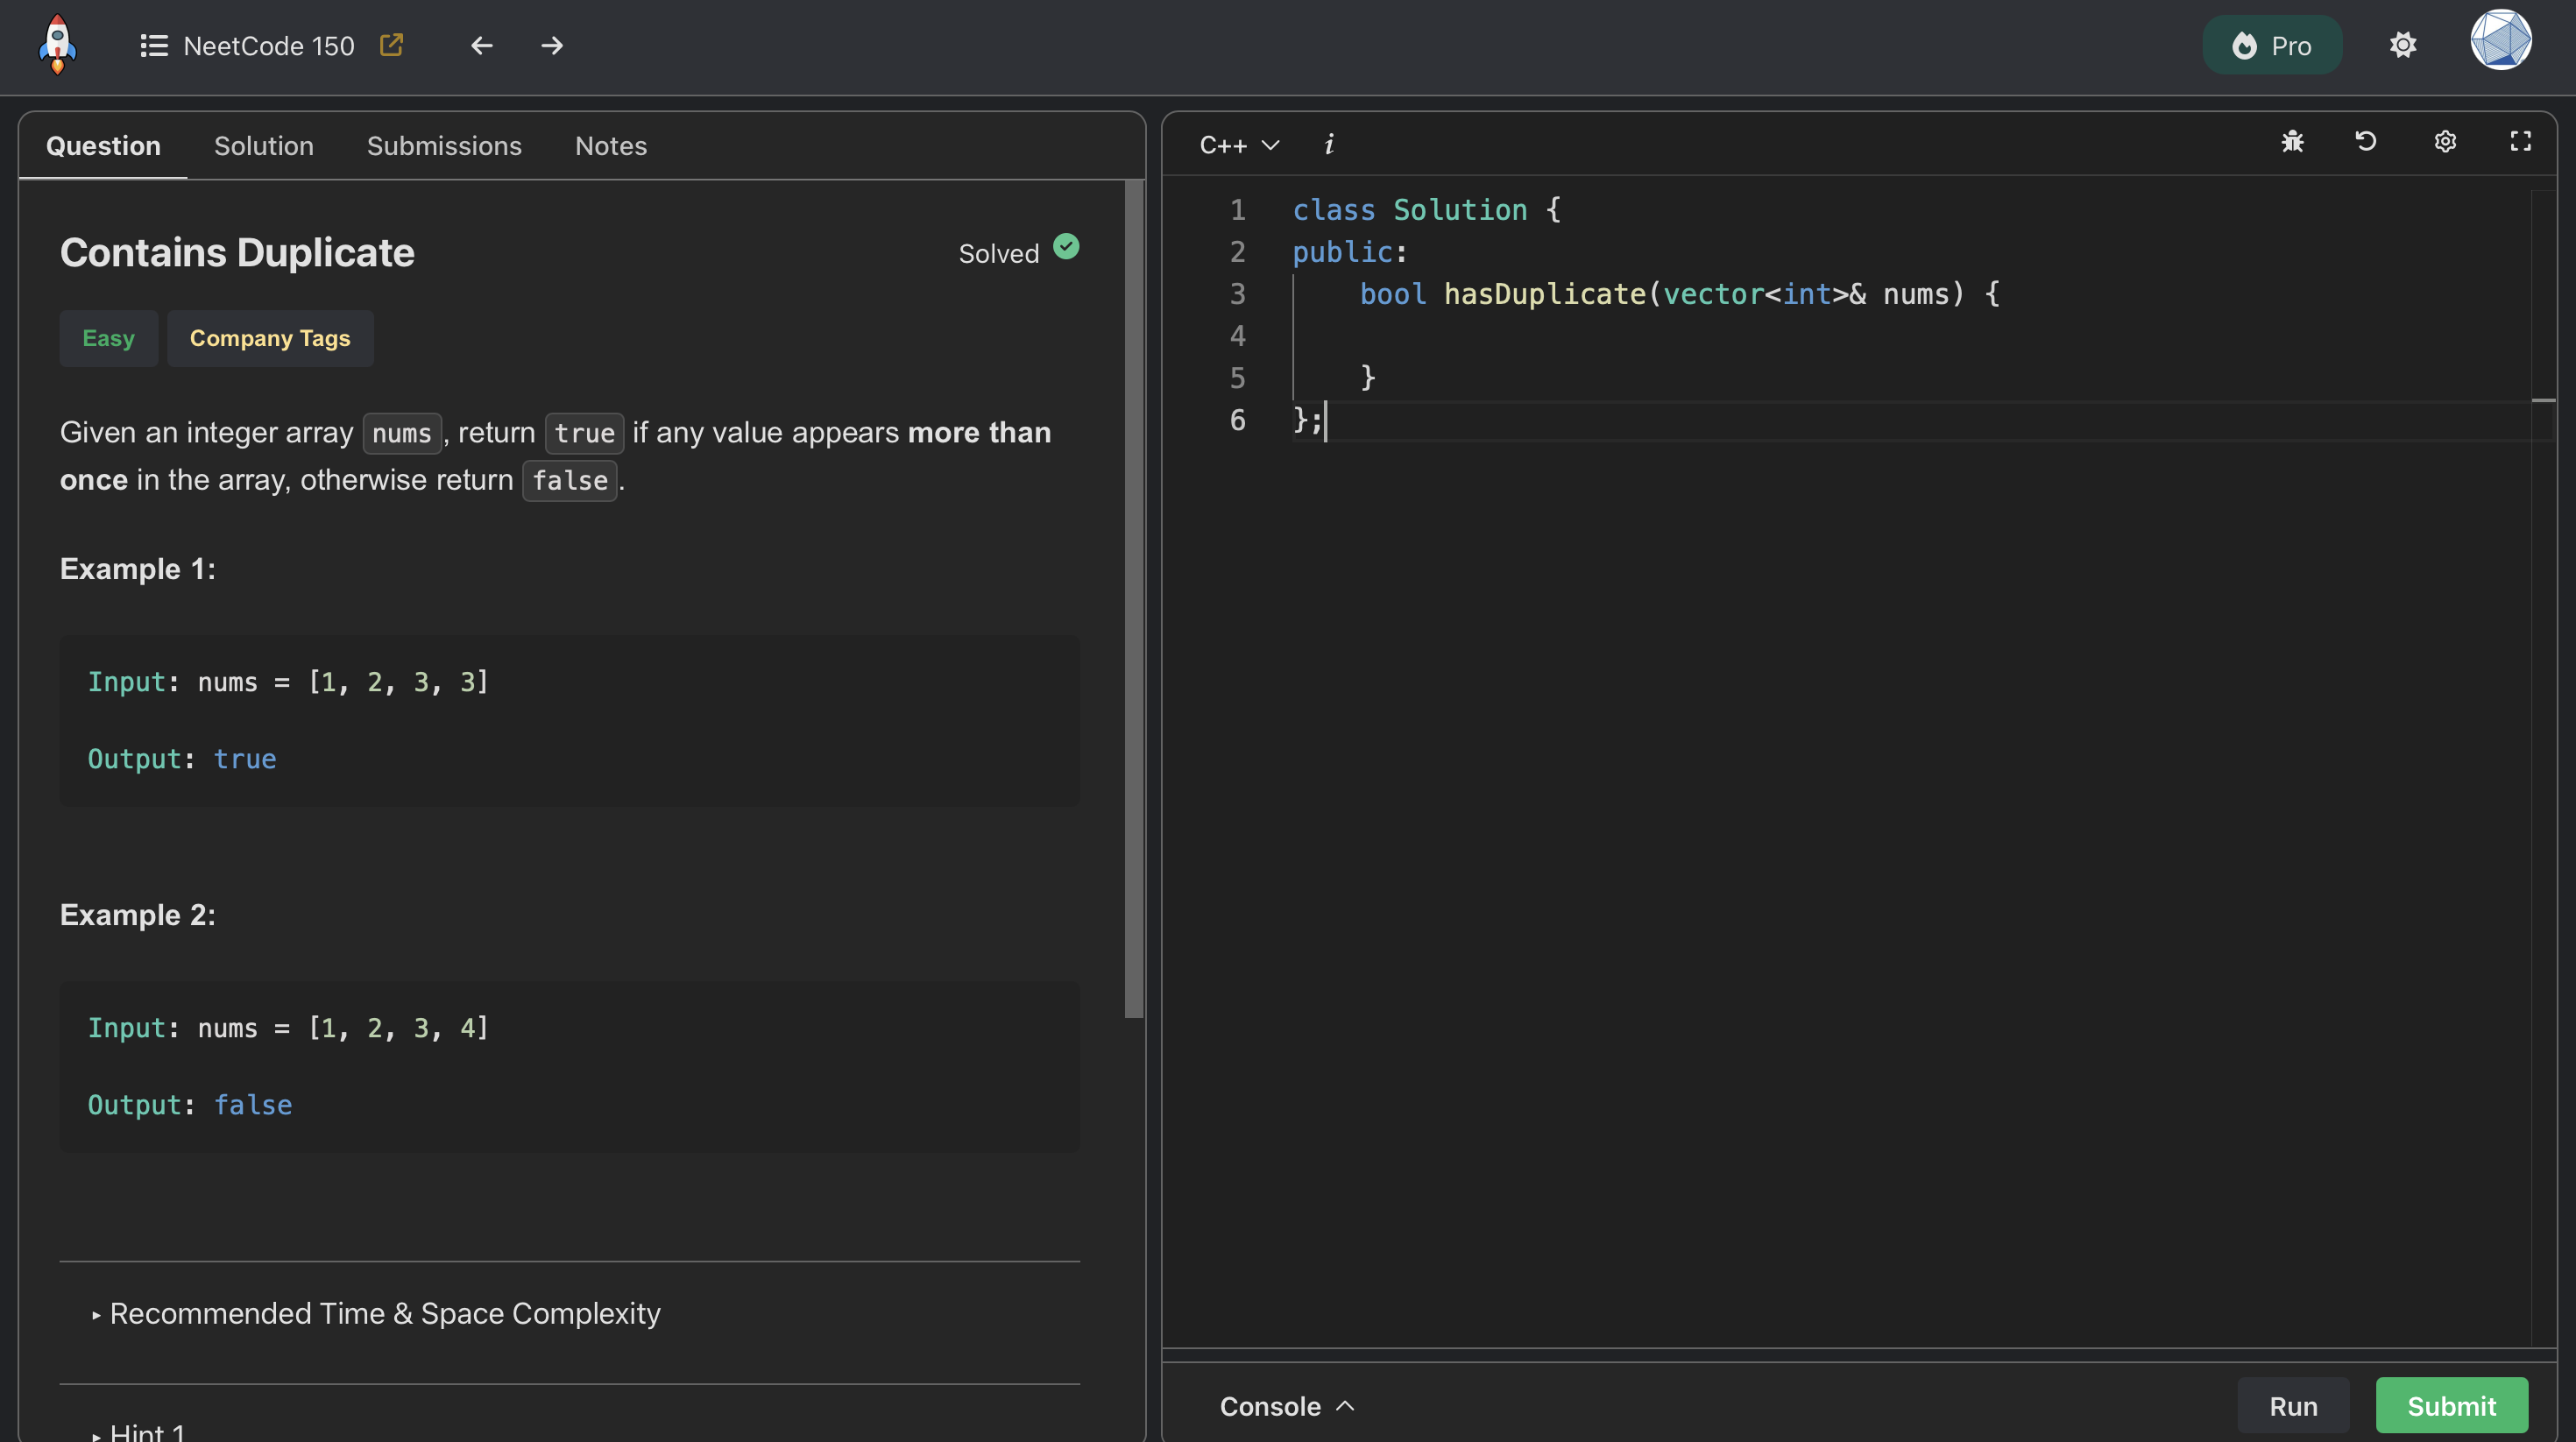
\includegraphics[width=0.95\textwidth]{NeetCodeProblem1.png}
\caption{Problem 1: Contains Duplicate - Given an array of integers, determine if any value appears at least twice}
\label{fig:problem1}
\end{figure}

\clearpage

\subsection{First Attempt and Why It Was Incorrect}

In my initial attempt, I began by examining the function signature:

\begin{lstlisting}[language=C++]
bool hasDuplicate(vector<int>& nums)
\end{lstlisting}

I correctly understood that the function returns a boolean value, meaning it must return either \texttt{true} or \texttt{false} depending on whether a duplicate exists in the input. I also understood that \texttt{vector<int>} represents a dynamic array of integers, and that the parameter name \texttt{nums} is simply what we call this array inside the function. Additionally, I did have a correct conceptual understanding of references: the ampersand (\texttt{\&}) indicates that the vector is passed by reference, allowing the function to access the original data directly without copying it, which improves efficiency.

The issue in my first attempt was not with understanding the function signature but with the approach I considered for solving the problem. I initially thought of comparing each integer in the vector with every other integer. Although this brute-force approach would eventually detect a duplicate, it requires nested loops and runs in $O(n^2)$ time. This does not meet the problem's requirement of achieving $O(n)$ time complexity. I recognized that this naive method was inefficient but had not yet identified the appropriate data structure or strategy needed to reach the desired complexity.

Thus, the main flaw in my first attempt was the time complexity of the solution method, not a misunderstanding of the function's return type or the use of references.

\section{Top K Frequent Elements}

% Problem description, approach, and solution

\section{Product of Array Except Self}

% Problem description, approach, and solution

\section{Valid Sudoku}

% Problem description, approach, and solution

\section{Encode and Decode Strings}

% Problem description, approach, and solution

\section{Longest Consecutive Sequence}

% Problem description, approach, and solution

\chapter{Two Pointers}

\section{Valid Palindrome}

% Problem description, approach, and solution

\section{Two Sum II}

% Problem description, approach, and solution

\section{3Sum}

% Problem description, approach, and solution

\section{Container With Most Water}

% Problem description, approach, and solution

\section{Trapping Rain Water}

% Problem description, approach, and solution

\chapter{Sliding Window}

\section{Best Time to Buy and Sell Stock}

% Problem description, approach, and solution

\section{Longest Substring Without Repeating Characters}

% Problem description, approach, and solution

\section{Longest Repeating Character Replacement}

% Problem description, approach, and solution

\section{Minimum Window Substring}

% Problem description, approach, and solution

\chapter{Stack}

\section{Valid Parentheses}

% Problem description, approach, and solution

\section{Min Stack}

% Problem description, approach, and solution

\section{Evaluate Reverse Polish Notation}

% Problem description, approach, and solution

\section{Generate Parentheses}

% Problem description, approach, and solution

\section{Daily Temperatures}

% Problem description, approach, and solution

\section{Car Fleet}

% Problem description, approach, and solution

\section{Largest Rectangle in Histogram}

% Problem description, approach, and solution

\chapter{Binary Search}

\section{Binary Search}

% Problem description, approach, and solution

\section{Search a 2D Matrix}

% Problem description, approach, and solution

\section{Koko Eating Bananas}

% Problem description, approach, and solution

\section{Find Minimum in Rotated Sorted Array}

% Problem description, approach, and solution

\section{Search in Rotated Sorted Array}

% Problem description, approach, and solution

\section{Time Based Key-Value Store}

% Problem description, approach, and solution

\section{Median of Two Sorted Arrays}

% Problem description, approach, and solution

\chapter{Linked List}

\section{Reverse Linked List}

% Problem description, approach, and solution

\section{Merge Two Sorted Lists}

% Problem description, approach, and solution

\section{Reorder List}

% Problem description, approach, and solution

\section{Remove Nth Node From End of List}

% Problem description, approach, and solution

\section{Copy List with Random Pointer}

% Problem description, approach, and solution

\section{Add Two Numbers}

% Problem description, approach, and solution

\section{Linked List Cycle}

% Problem description, approach, and solution

\section{Find the Duplicate Number}

% Problem description, approach, and solution

\section{LRU Cache}

% Problem description, approach, and solution

\section{Merge K Sorted Lists}

% Problem description, approach, and solution

\section{Reverse Nodes in K-Group}

% Problem description, approach, and solution

\chapter{Trees}

\section{Invert Binary Tree}

% Problem description, approach, and solution

\section{Maximum Depth of Binary Tree}

% Problem description, approach, and solution

\section{Diameter of Binary Tree}

% Problem description, approach, and solution

\section{Balanced Binary Tree}

% Problem description, approach, and solution

\section{Same Tree}

% Problem description, approach, and solution

\section{Subtree of Another Tree}

% Problem description, approach, and solution

\section{Lowest Common Ancestor of a Binary Search Tree}

% Problem description, approach, and solution

\section{Binary Tree Level Order Traversal}

% Problem description, approach, and solution

\section{Binary Tree Right Side View}

% Problem description, approach, and solution

\section{Count Good Nodes in Binary Tree}

% Problem description, approach, and solution

\section{Validate Binary Search Tree}

% Problem description, approach, and solution

\section{Kth Smallest Element in a BST}

% Problem description, approach, and solution

\section{Construct Binary Tree from Preorder and Inorder Traversal}

% Problem description, approach, and solution

\section{Binary Tree Maximum Path Sum}

% Problem description, approach, and solution

\section{Serialize and Deserialize Binary Tree}

% Problem description, approach, and solution

\chapter{Tries}

\section{Implement Trie}

% Problem description, approach, and solution

\section{Design Add and Search Words Data Structure}

% Problem description, approach, and solution

\section{Word Search II}

% Problem description, approach, and solution

\chapter{Heap / Priority Queue}

\section{Kth Largest Element in a Stream}

% Problem description, approach, and solution

\section{Last Stone Weight}

% Problem description, approach, and solution

\section{K Closest Points to Origin}

% Problem description, approach, and solution

\section{Kth Largest Element in an Array}

% Problem description, approach, and solution

\section{Task Scheduler}

% Problem description, approach, and solution

\section{Design Twitter}

% Problem description, approach, and solution

\section{Find Median from Data Stream}

% Problem description, approach, and solution

\chapter{Backtracking}

\section{Subsets}

% Problem description, approach, and solution

\section{Combination Sum}

% Problem description, approach, and solution

\section{Permutations}

% Problem description, approach, and solution

\section{Subsets II}

% Problem description, approach, and solution

\section{Combination Sum II}

% Problem description, approach, and solution

\section{Word Search}

% Problem description, approach, and solution

\section{Palindrome Partitioning}

% Problem description, approach, and solution

\section{Letter Combinations of a Phone Number}

% Problem description, approach, and solution

\section{N-Queens}

% Problem description, approach, and solution

\end{document}
